\chapter{Multi-Objective Optimization}
\todoChapter{%
  {\color{gray}10\% complete. Goal 80\% completion date: January 20, 2023}\\
  Notes: Clean up this section. Add more information.
}

\begin{outcome}
\begin{itemize}
    \item Define multi-objective optimization problems
    \item Discuss solutions in terms of the \emph{Pareto Frontier}
    \item Explore approaches for finding the Pareto Frontier
    \item Use software to solve for or approximate the Pareto Frontier
\end{itemize}
\end{outcome}



\section{Introduction to Multi-Objective Optimization}

In many real-world problems, decision makers must balance competing objectives. Rather than optimizing a single quantity, we seek solutions that trade off different goals — cost vs. quality, speed vs. safety, efficiency vs. equity, and so on. This leads to the field of \emph{multi-objective optimization} (MOO), which provides a framework for identifying and analyzing such trade-offs.

To illustrate this, consider a simple inventory and production planning problem over a fixed horizon of \(T = 10\) periods. Let \(x_t\) denote the quantity produced in period \(t\), \(s_t\) the inventory carried over after period \(t\), and \(d_t\) the demand to be satisfied during that period. The system begins with \(s_0 = 5\) units of initial inventory. Production costs \(c^p_t\) vary by time, while holding inventory incurs a fixed per-unit cost \(c^h\).

\textbf{The inventory balance constraint} for each period is:
\[
s_t = s_{t-1} + x_t - d_t \quad \text{for all } t = 1,\ldots,T
\]

\textbf{The objective function} (single-objective version) is to minimize total cost:
\[
\min \sum_{t=1}^{T} \left( c^p_t x_t + c^h s_t \right)
\]

However, holding inventory is not just costly — it also introduces risk. Products may be damaged, stolen, or become obsolete. To capture this additional concern, we define a \textbf{risk function} that models the expected loss due to stored inventory:
\[
r(s_t) = c_r \left(1 - e^{-\beta s_t}\right)
\]
where \(c_r\) is the maximum risk cost and \(\beta\) is a sensitivity parameter. This function grows quickly at first, but saturates as inventory increases, reflecting that the marginal risk of storing more units diminishes with protective measures (e.g., insurance, security systems).

\begin{figure}[h]
    \centering
    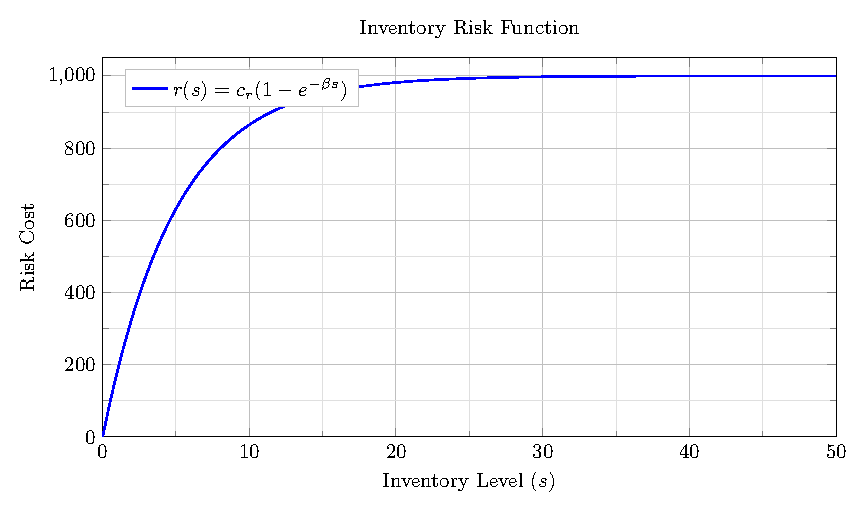
\includegraphics[width=0.65\textwidth]{Figures/risk-plot.pdf}
    \caption{Inventory risk cost as a function of inventory level.}
\end{figure}

Now we face a \textbf{multi-objective problem}: we want to minimize both total cost and maximum risk incurred across the planning horizon. These objectives are in tension: reducing risk requires keeping inventory low, which often means producing more frequently at higher cost.

To explore the trade-off, we solve the problem repeatedly with varying upper bounds on inventory (i.e., limiting \(s_t \leq R\)), and for each value compute:
\begin{itemize}
    \item The optimal total cost (production + holding),
    \item The maximum risk experienced across all periods, computed as \( \max_t r(s_t) \).
\end{itemize}

The resulting plot shows the \emph{Pareto frontier} of non-dominated solutions — those for which no other solution achieves both a lower cost and lower risk.

\begin{figure}[h]
    \centering
    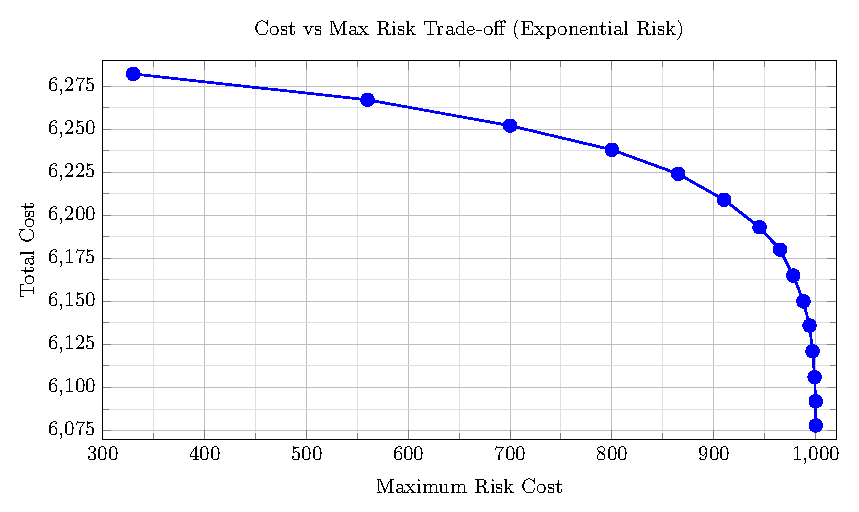
\includegraphics[width=0.7\textwidth]{Figures/pareto-curve.pdf}
    \caption{Trade-off between total cost and maximum inventory risk.}
\end{figure}

This example illustrates the essence of multi-objective optimization: generating and analyzing a spectrum of solutions that offer different balances between competing goals. In practice, decision makers select among these using domain knowledge, regulatory limits, or stakeholder preferences.





%\section{Introduction to Multi-Objective Optimization and the Pareto Frontier}
%
%Multi-objective optimization (MOO) involves simultaneously optimizing two or more conflicting objectives subject to certain constraints. In many real-world applications, improving one objective often leads to a trade-off in another. One key concept is the \emph{Pareto Frontier} (or \emph{Pareto Front}), which is the set of all solutions that cannot improve any objective without worsening at least one other objective.  
%
%\subsection{Motivating Example: Furniture Manufacturer}
%
%Consider a high-end furniture manufacturer which builds dining tables and chairs out of expensive bocote and rosewood:
%
%\begin{figure}[h]
%    \centering
%    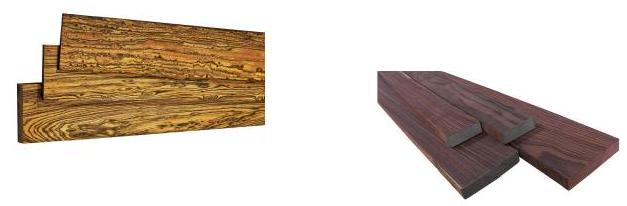
\includegraphics[width=0.5\textwidth]{optimization/multi-objective/images/2022_02_28_634e8079070800ac7e3cg-02}
%    \caption{Tables and chairs made from bocote and rosewood.}
%\end{figure}
%
%The manufacturer has an ongoing deal with a foreign sawmill which supplies them with 960 and 200 board-feet (bdft) of bocote and rosewood respectively each month. A single table requires 80~bdft of bocote and 20~bdft of rosewood, while each chair requires 20~bdft of bocote and 10~bdft of rosewood. We denote the number of tables to be produced as \(x\) and the number of chairs as \(y\). The feasible production set \(P\) is given by:
%
%\[
%\begin{aligned}
%P = \{(x,y) \in \mathbb{R}^2 :\,& 80x + 20y \le 960,\\
%                                   & 12x + 10y \le 200,\\
%                                   & x, y \ge 0 \}.
%\end{aligned}
%\]
%
%\begin{figure}[h]
%    \centering
%    
%    \begin{tikzpicture}
%  \begin{axis}[
%    xlabel={number of tables ($x$)},
%    ylabel={number of chairs ($y$)},
%    axis lines=left,
%    xmin=0, xmax=13,
%    ymin=0, ymax=21,
%    xtick={0,2,4,6,8,10,12},
%    ytick={0,5,10,15,20},
%    width=12cm,
%    height=9cm,
%    grid=both,
%    enlargelimits=false,
%  ]
%
%  % Feasible region (blue fill)
%  \addplot[fill=blue!30, draw=blue, opacity = 0.3, thick] coordinates {
%    (0,0)
%    (0,20)
%    (10,8)
%    (12,0)
%    (0,0)
%  };
%
%  % Constraint lines
%  \addplot[domain=0:12, thick, blue] {48 - 4*x}; % 80x + 20y = 960
%  \addplot[domain=0:12, thick, blue] {20 - 1.2*x}; % 12x + 10y = 200
%
%  % Integer points in feasible region
%%  \foreach \pt in {
%%    (0,0), (0,20), (10,8), (12,0),
%%    (1,18), (2,16), (3,14), (4,12), (5,10), (6,8), (7,6), (8,4), (9,2), (10,0)
%%  } {
%%    \addplot[only marks, mark=*, mark size=2pt, black] coordinates {\pt};
%%  }
%    % Objective function lines (example)
%
%
%  \end{axis}
%\end{tikzpicture}
%
%
%    %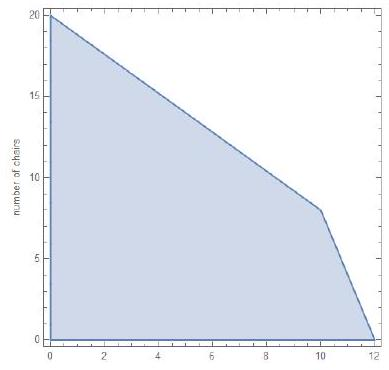
\includegraphics[width=0.5\textwidth]{optimization/multi-objective/images/2022_02_28_634e8079070800ac7e3cg-03}
%    \caption{Feasible region for the furniture production problem.}
%\end{figure}
%
%\subsubsection{First Objective: Profit Maximization}
%
%Suppose each table sells for \$7000 and each chair sells for \$1500. We want to maximize profit:
%\[
%F(x,y) = 8000x + 2000y
%\]
%over the feasible region \(P\). In the language of linear programming:
%\[
%\text{Maximize } 8000x + 2000y
%\]
%subject to
%\[
%80x + 20y \le 960, \quad
%12x + 10y \le 200, \quad
%x, y \ge 0.
%\]
%
%Sometimes, to simplify arithmetic, the objective can be scaled down (e.g., divide the profit coefficients by 2000). Let us define a scaled objective:
%\[
%w = 4x + y.
%\]
%Then our constraints become:
%\[
%4x + y \le 48, \quad
%6x + 5y \le 100, \quad
%x, y \ge 0.
%\]
%We introduce slack variables \(s_1, s_2\) to convert the inequalities into equalities:
%\[
%\begin{aligned}
%4x + y + s_1 &= 48,\\
%6x + 5y + s_2 &= 100,\\
%x,\,y,\,s_1,\,s_2 &\ge 0.
%\end{aligned}
%\]
%
%\paragraph{Setting up the Simplex Dictionary}
%
%Instead of forming a traditional simplex \emph{tableau}, we will use \emph{simplex dictionaries}. In the initial dictionary, we represent the (scaled) objective \(w\) in terms of the decision variables. The dictionary often has the form:
%\[
%\begin{aligned}
%w \;&=\; 4x + y,\\
%s_1 \;&=\; 48 \;-\; 4x \;-\; y,\\
%s_2 \;&=\; 100 \;-\; 6x \;-\; 5y.
%\end{aligned}
%\]
%We seek to \emph{maximize} \(w\). At each iteration of the simplex method, we pivot to rewrite the dictionary so that one basic variable appears on the left side for each equation, and we update the expression for \(w\) accordingly. Eventually, we find an optimal basic feasible solution.
%
%Solving via dictionaries (just as with tableaus) reveals an optimal profit at \(\,x=12,\; y=0\). However, \emph{there are multiple solutions} on the boundary that achieve the same maximum revenue. 
%
%\begin{figure}[h]
%    \centering
%        \begin{tikzpicture}
%  \begin{axis}[
%    xlabel={number of tables ($x$)},
%    ylabel={number of chairs ($y$)},
%    axis lines=left,
%    xmin=0, xmax=13,
%    ymin=0, ymax=21,
%    xtick={0,2,4,6,8,10,12},
%    ytick={0,5,10,15,20},
%    width=12cm,
%    height=9cm,
%    grid=both,
%    enlargelimits=false,
%  ]
%
%  % Feasible region (blue fill)
%  \addplot[fill=blue!30, draw=blue, opacity = 0.3, thick] coordinates {
%    (0,0)
%    (0,20)
%    (10,8)
%    (12,0)
%    (0,0)
%  };
%  
%    %\addplot[fill=blue!70, draw=blue, opacity = 0.3, thick] coordinates {
%%    (8.5,0)
%%    (5,14)
%%    (10,8)
%%    (12,0)
%%    (8.5,0)
%%  };
%
%  % Constraint lines
%  \addplot[domain=0:12, thick, blue] {48 - 4*x}; % 80x + 20y = 960
%  \addplot[domain=0:12, thick, blue] {20 - 1.2*x}; % 12x + 10y = 200
%
%  % Integer points in feasible region
%%  \foreach \pt in {
%%    (0,0), (0,20), (10,8), (12,0),
%%    (1,18), (2,16), (3,14), (4,12), (5,10), (6,8), (7,6), (8,4), (9,2), (10,0)
%%  } {
%%    \addplot[only marks, mark=*, mark size=2pt, black] coordinates {\pt};
%%  }
%    % Objective function lines (example)
%\foreach \z in {5,10,...,60}{
%    \addplot[dashed,gray, domain=0:13, samples=2] {(\z - 4*x)};
%}
%
%
%  \end{axis}
%\end{tikzpicture}
%    %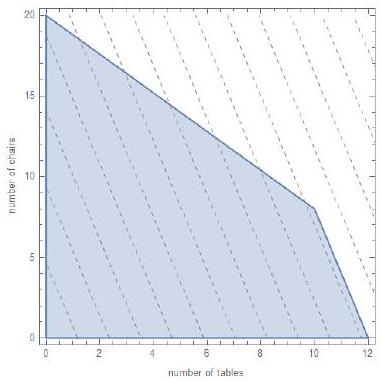
\includegraphics[width=0.5\textwidth]{optimization/multi-objective/images/2022_02_28_634e8079070800ac7e3cg-05}
%    \caption{Optimal solutions on the boundary for the profit objective.}
%\end{figure}
%
%\paragraph{Are these solutions really equivalent?}
%Yes---in terms of revenue, they all give the same maximum value. But let’s see how introducing a second objective changes the picture.
%
%\subsubsection{Second Objective: Reducing Waste of Rosewood}
%
%A new manager notices that table production wastes nearly 10 bdft of rosewood per table, while chair production wastes only 2 bdft per chair. She wants to break the tie among the multiple revenue-maximizing solutions by introducing a secondary objective function to \emph{minimize} the waste:
%\[
%w(x,y) = 10x + 2y.
%\]
%She focuses on the subset of the feasible region that yields maximum revenue and sets up a small linear program restricting us to the line segment of profit-optimal solutions. In this case, that segment lies between the extreme points \((12,0)\) and \((10,8)\). Thus, she solves:
%\[
%\begin{aligned}
%\text{Minimize } &\, 10x + 2y \\
%\text{subject to } &\, 80x + 20y = 960,\\
%&\, x \in [10,12], \quad y \in [0,8].
%\end{aligned}
%\]
%Among the two corner points \((12,0)\) and \((10,8)\), \((10,8)\) yields less rosewood waste (while still maintaining the same revenue). 
%
%This approach is known as the \emph{Ordered Criteria} or \emph{Lexicographic} method, where objectives are prioritized in a strict order: first maximize profit, then among those maximizers, minimize waste.
%
%\subsubsection{Allowing Some Loss of Profit}
%
%After a few months, the manager convinces the owners that reducing waste is worth some loss in profit. They agree to a 30\% loss in revenue; thus, the manager uses a new model:
%
%\[
%\begin{aligned}
%&\text{Minimize } 10x + 2y,\\
%&\text{subject to } \quad 8000x + 2000y \;\ge\; \alpha \cdot 96000, \\
%&\qquad 80x + 20y \;\le\; 960, \\
%&\qquad 12x + 10y \;\le\; 200, \\
%&\qquad x, y \;\ge\; 0,
%\end{aligned}
%\]
%where \(\alpha = 0.7\). This ensures the chosen solution retains at least \(70\%\) of the maximum possible revenue while minimizing waste. This \emph{rollover} or \emph{benchmark} method requires knowledge of the optimal value of the first objective (the maximum revenue).
%
%\begin{figure}[h]
%    \centering
%            \begin{tikzpicture}
%  \begin{axis}[
%    xlabel={number of tables ($x$)},
%    ylabel={number of chairs ($y$)},
%    axis lines=left,
%    xmin=0, xmax=13,
%    ymin=0, ymax=21,
%    xtick={0,2,4,6,8,10,12},
%    ytick={0,5,10,15,20},
%    width=12cm,
%    height=9cm,
%    grid=both,
%    enlargelimits=false,
%  ]
%
%  % Feasible region (blue fill)
%  \addplot[fill=blue!30, draw=blue, opacity = 0.3, thick] coordinates {
%    (0,0)
%    (0,20)
%    (10,8)
%    (12,0)
%    (0,0)
%  };
%  
%    \addplot[fill=blue!70, draw=blue, opacity = 0.3, thick] coordinates {
%    (8.5,0)
%    (5,14)
%    (10,8)
%    (12,0)
%    (8.5,0)
%  };
%
%  % Constraint lines
%  \addplot[domain=0:12, thick, blue] {48 - 4*x}; % 80x + 20y = 960
%  \addplot[domain=0:12, thick, blue] {20 - 1.2*x}; % 12x + 10y = 200
%
%  % Integer points in feasible region
%%  \foreach \pt in {
%%    (0,0), (0,20), (10,8), (12,0),
%%    (1,18), (2,16), (3,14), (4,12), (5,10), (6,8), (7,6), (8,4), (9,2), (10,0)
%%  } {
%%    \addplot[only marks, mark=*, mark size=2pt, black] coordinates {\pt};
%%  }
%    % Objective function lines (example)
%%\foreach \z in {5,10,...,60}{
%%    \addplot[dashed,gray, domain=0:13, samples=2] {(\z - 4*x)};
%%}
%\foreach \z in {5,10,...,60}{
%    \addplot[dashed,purple, domain=0:13, samples=2] {(\z - 5*x)};
%}
%
%  \end{axis}
%\end{tikzpicture}%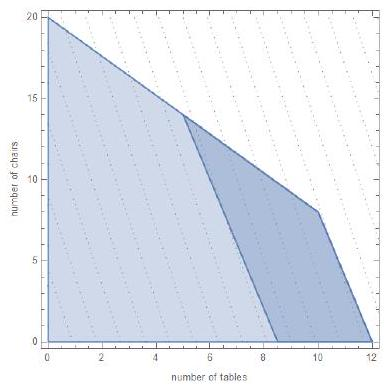
\includegraphics[width=0.5\textwidth]{optimization/multi-objective/images/2022_02_28_634e8079070800ac7e3cg-10}
%    \caption{Feasible set with revenue constrained to at least 70\% of the maximum.}
%\end{figure}
%
%Interestingly, the new solution (with \(\alpha=0.7\)) might not be an extreme point of the \emph{original} feasible region, but it is an extreme point of the \emph{subset} of solutions constrained by \(8000x + 2000y \ge 0.7 \times 96000\).
%
%
%
%\subsection{Pareto Optimality and the Pareto Frontier}
%
%In many real-world optimization problems, we must balance multiple conflicting objectives. For instance, a transportation planner might seek to minimize both cost and environmental impact, or a manufacturer might want to maximize both product quality and production efficiency. In such cases, there is often no single solution that is best across all objectives. Instead, we aim to identify a set of \emph{efficient} solutions where improvement in one objective would necessarily lead to deterioration in another. These are known as \textbf{Pareto optimal solutions}, and collectively they form the \textbf{Pareto frontier}, which represents the trade-offs between competing objectives.
%
%\begin{definition}{Pareto Optimal}{}
%Given a set \(P\) and several objective functions \(f_i: P \to \mathbb{R}\) that we seek to \emph{maximize}, a point \(\mathbf{x} \in P\) is called \emph{Pareto Optimal} (or \emph{Efficient}) if there is no \(\overline{\mathbf{x}} \in P\) such that:
%\[
%\begin{aligned}
%& f_i(\overline{\mathbf{x}}) > f_i(\mathbf{x}) \text{ for some } i, \\
%& f_j(\overline{\mathbf{x}}) \ge f_j(\mathbf{x}) \text{ for all } j \ne i.
%\end{aligned}
%\]
%In other words, you cannot make any objective strictly better without making at least one other objective strictly worse. The \emph{Pareto Frontier} is the set of all such Pareto optimal solutions.
%\end{definition}
%
%We will discuss some of the main approaches for multi-objective optimization summarized in this table here.
%
%\begin{table}[h]
%\centering
%\caption{Summary of Multi-Objective Optimization Methods}
%\renewcommand{\arraystretch}{1.3}
%\begin{tabular}{|l|p{4.2cm}|p{3.5cm}|p{3.5cm}|}
%\hline
%\textbf{Method} & \textbf{Key Idea} & \textbf{Pros} & \textbf{Cons} \\
%\hline
%\textbf{Weighted Sum} & Combine objectives into a single scalar using a weighted sum & Simple and computationally efficient & May miss Pareto-optimal solutions in non-convex regions \\
%\hline
%\textbf{Lexicographic} & Prioritize objectives in strict order; optimize one at a time & Matches real-world priorities; no need to choose weights & Does not explore trade-offs or provide a frontier \\
%\hline
%\textbf{Epsilon-Constraint} & Optimize one objective, convert others into constraints with adjustable bounds & Explores full frontier, even non-convex parts & Requires repeated solves and tuning of $\varepsilon$ values \\
%\hline
%\textbf{Goal Programming} & Minimize weighted deviation from target values (goals) for each objective & Flexible, intuitive, and useful in decision-making contexts & Can be sensitive to goal setting and weights \\
%\hline
%\end{tabular}
%\end{table}



\begin{figure}[h]
    \centering
    
            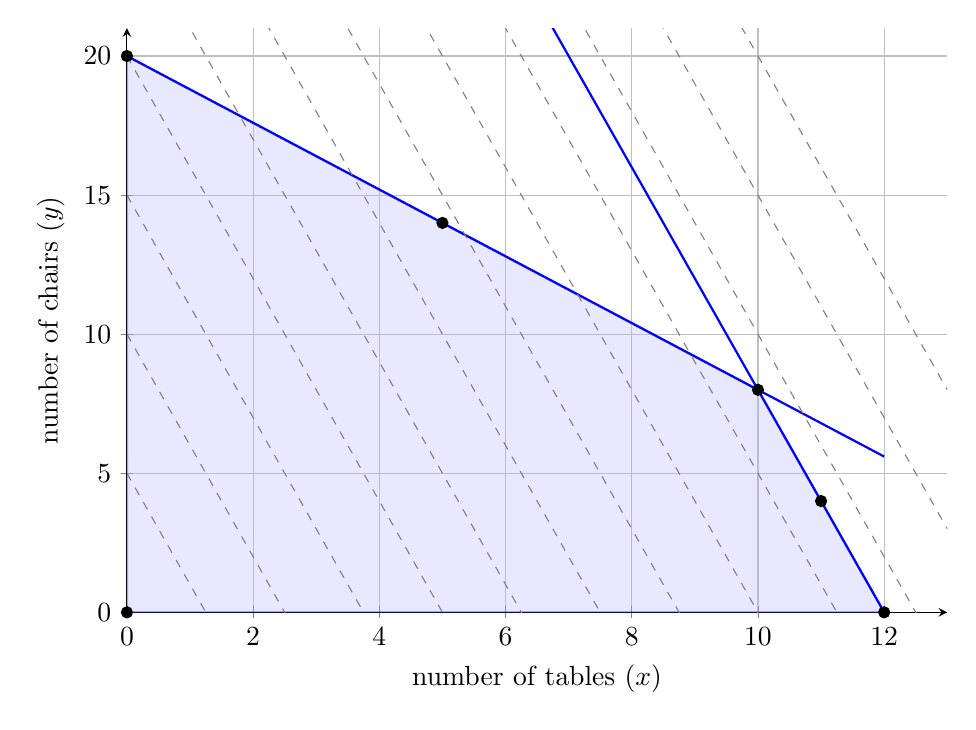
\begin{tikzpicture}
  \begin{axis}[
    xlabel={number of tables ($x$)},
    ylabel={number of chairs ($y$)},
    axis lines=left,
    xmin=0, xmax=13,
    ymin=0, ymax=21,
    xtick={0,2,4,6,8,10,12},
    ytick={0,5,10,15,20},
    width=12cm,
    height=9cm,
    grid=both,
    enlargelimits=false,
  ]

  % Feasible region (blue fill)
  \addplot[fill=blue!30, draw=blue, opacity = 0.3, thick] coordinates {
    (0,0)
    (0,20)
    (10,8)
    (12,0)
    (0,0)
  };
  
  % Constraint lines
  \addplot[domain=0:12, thick, blue] {48 - 4*x}; % 80x + 20y = 960
  \addplot[domain=0:12, thick, blue] {20 - 1.2*x}; % 12x + 10y = 200

  % Integer points in feasible region
  \foreach \pt in {
    (0,0), (0,20), (10,8), (12,0),
    (5,14), (11,4)
  } {
    \addplot[only marks, mark=*, mark size=2pt, black] coordinates {\pt};
  }
    % Objective function lines (example)
\foreach \z in {5,10,...,60}{
    \addplot[dashed,gray, domain=0:13, samples=2] {(\z - 4*x)};
}


  \end{axis}
\end{tikzpicture}

    %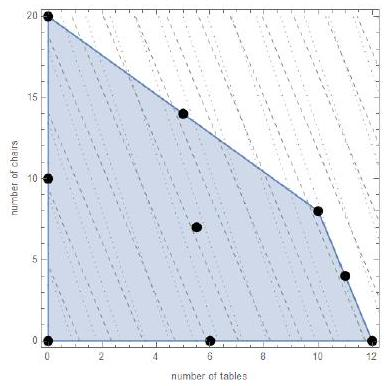
\includegraphics[width=0.5\textwidth]{optimization/multi-objective/images/2022_02_28_634e8079070800ac7e3cg-13}
    \caption{Identifying the Pareto frontier among possible solutions.}
\end{figure}

\subsection{Further Methods for Multi-Objective Optimization}

\paragraph{Scalarization (Weighted Sum) Method}

Another common approach is \emph{scalarization}: pick some constant \(\lambda \in [0,1]\) and form a single objective by combining the two objectives linearly:
\[
\begin{aligned}
&\text{Minimize } \lambda (8000x + 2000y) + (1-\lambda)(10x + 2y)\\
&\text{subject to }\, 80x + 20y \le 960, \\
&\qquad\qquad 12x + 10y \le 200, \\
&\qquad\qquad x, y \ge 0.
\end{aligned}
\]
By varying \(\lambda\), one can trace out (part of) the Pareto frontier; however, the method may miss some \emph{non-convex} portions of the frontier in more complex problems.  



\section{Multi-Objective Optimization and the Pareto Frontier}

Multi-objective optimization (MOO) involves simultaneously optimizing two or more conflicting objectives subject to certain constraints. In many real-world applications, improving one objective often leads to a trade-off in another. A central concept in MOO is the \emph{Pareto Frontier} (or \emph{Pareto Front}), which consists of all solutions for which no objective can be improved without worsening at least one other.

\paragraph{Motivating Example: Furniture Manufacturer}

Consider a high-end furniture manufacturer that builds dining tables and chairs from expensive bocote and rosewood:

\begin{figure}[h]
    \centering
    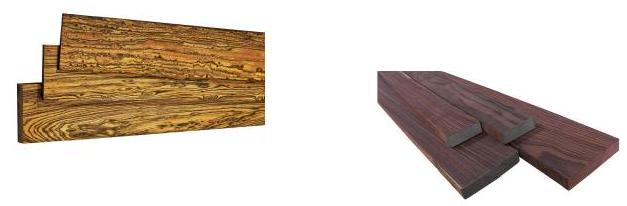
\includegraphics[width=0.5\textwidth]{optimization/multi-objective/images/2022_02_28_634e8079070800ac7e3cg-02}
    \caption{Tables and chairs made from bocote and rosewood.}
\end{figure}

The manufacturer receives 960 board-feet (bdft) of bocote and 200 bdft of rosewood per month. Each table requires 80~bdft of bocote and 20~bdft of rosewood; each chair requires 20~bdft of bocote and 10~bdft of rosewood. Let \(x\) denote the number of tables and \(y\) the number of chairs produced. The feasible production set \(P\) is given by:

\[
\begin{aligned}
P = \{(x,y) \in \mathbb{R}^2 :\,& 80x + 20y \le 960,\\
                                   & 12x + 10y \le 200,\\
                                   & x, y \ge 0 \}.
\end{aligned}
\]


\[
\begin{aligned}
P = \{(x,y) \in \mathbb{R}^2 :\,& 80x + 20y \le 960,\\
                                   & 12x + 10y \le 200,\\
                                   & x, y \ge 0 \}.
\end{aligned}
\]

\begin{figure}[h]
    \centering
    
    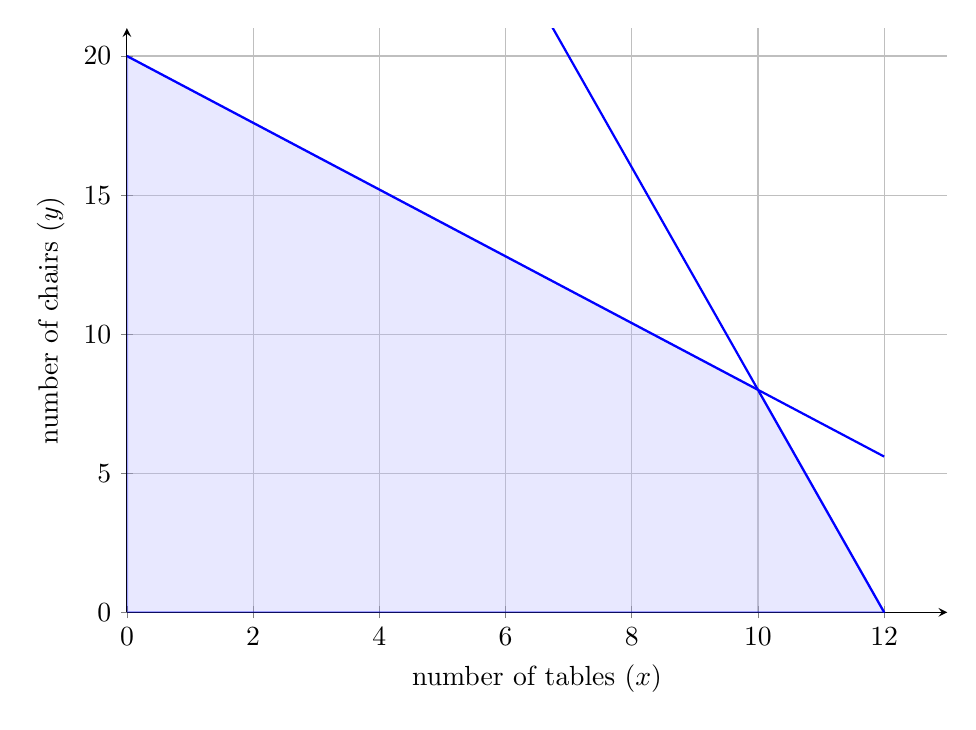
\begin{tikzpicture}
  \begin{axis}[
    xlabel={number of tables ($x$)},
    ylabel={number of chairs ($y$)},
    axis lines=left,
    xmin=0, xmax=13,
    ymin=0, ymax=21,
    xtick={0,2,4,6,8,10,12},
    ytick={0,5,10,15,20},
    width=12cm,
    height=9cm,
    grid=both,
    enlargelimits=false,
  ]

  % Feasible region (blue fill)
  \addplot[fill=blue!30, draw=blue, opacity = 0.3, thick] coordinates {
    (0,0)
    (0,20)
    (10,8)
    (12,0)
    (0,0)
  };

  % Constraint lines
  \addplot[domain=0:12, thick, blue] {48 - 4*x}; % 80x + 20y = 960
  \addplot[domain=0:12, thick, blue] {20 - 1.2*x}; % 12x + 10y = 200

  % Integer points in feasible region
%  \foreach \pt in {
%    (0,0), (0,20), (10,8), (12,0),
%    (1,18), (2,16), (3,14), (4,12), (5,10), (6,8), (7,6), (8,4), (9,2), (10,0)
%  } {
%    \addplot[only marks, mark=*, mark size=2pt, black] coordinates {\pt};
%  }
    % Objective function lines (example)


  \end{axis}
\end{tikzpicture}


    %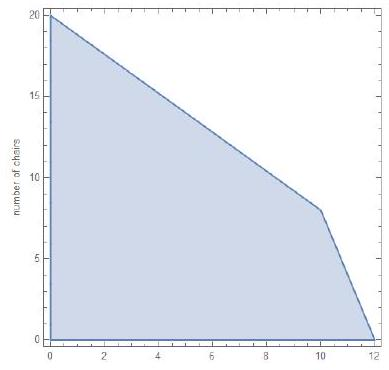
\includegraphics[width=0.5\textwidth]{optimization/multi-objective/images/2022_02_28_634e8079070800ac7e3cg-03}
    \caption{Feasible region for the furniture production problem.}
\end{figure}

Suppose each table earns \$8000 and each chair earns \$2000. The goal is to maximize revenue:

\[
\text{Maximize } 8000x + 2000y \quad \text{subject to } (x, y) \in P.
\]

Scaling the objective to \(w = 4x + y\), the feasible region remains the same but is easier to visualize. Solving this LP reveals multiple optimal solutions on the boundary from \((12, 0)\) to \((10, 8)\). These all yield the same profit, but they may differ in other criteria.

Now, suppose a new manager wants to minimize material waste—specifically, 10~bdft wasted per table and 2~bdft per chair:

\[
\text{Minimize } 10x + 2y \quad \text{subject to maximum revenue}.
\]

Restricting attention to the profit-optimal frontier and minimizing waste identifies \((10, 8)\) as preferable. This is an example of the \emph{lexicographic method}: optimize a primary objective, then refine solutions with a secondary one.

Alternatively, the manager may be willing to sacrifice some revenue. If they accept at least 70\% of maximum profit, they solve:

\[
\begin{aligned}
\text{Minimize } &\, 10x + 2y \\
\text{subject to } &\, 8000x + 2000y \ge 0.7 \times 96000,\\
&\, (x, y) \in P.
\end{aligned}
\]

\begin{figure}[h]
    \centering
            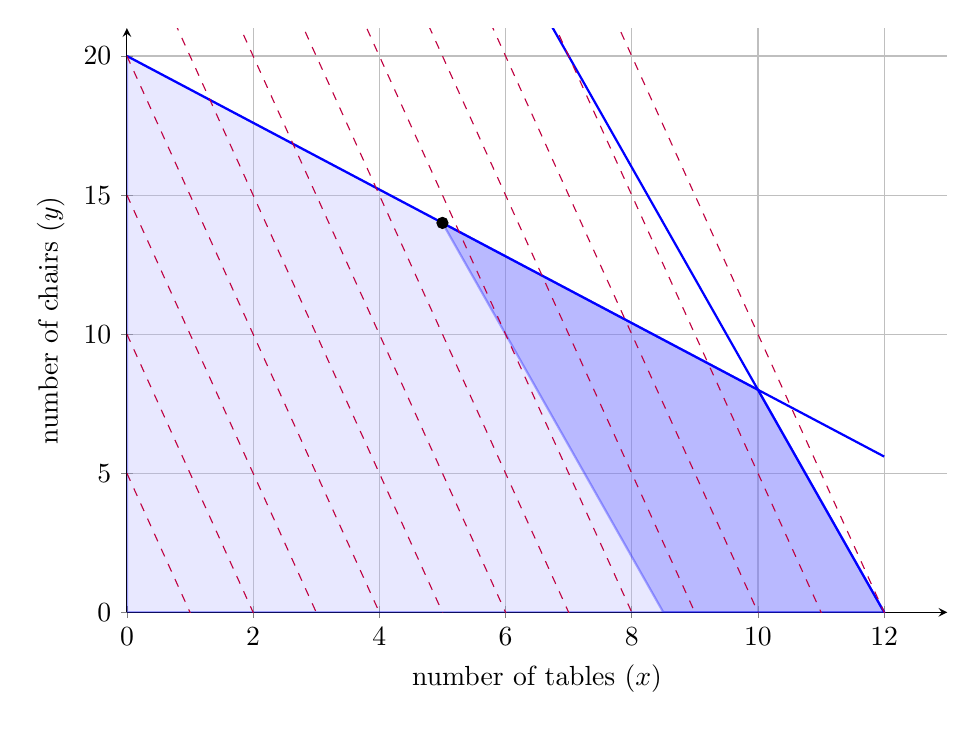
\begin{tikzpicture}
  \begin{axis}[
    xlabel={number of tables ($x$)},
    ylabel={number of chairs ($y$)},
    axis lines=left,
    xmin=0, xmax=13,
    ymin=0, ymax=21,
    xtick={0,2,4,6,8,10,12},
    ytick={0,5,10,15,20},
    width=12cm,
    height=9cm,
    grid=both,
    enlargelimits=false,
  ]

  % Feasible region (blue fill)
  \addplot[fill=blue!30, draw=blue, opacity = 0.3, thick] coordinates {
    (0,0)
    (0,20)
    (10,8)
    (12,0)
    (0,0)
  };
  
    \addplot[fill=blue!70, draw=blue, opacity = 0.3, thick] coordinates {
    (8.5,0)
    (5,14)
    (10,8)
    (12,0)
    (8.5,0)
  };

  % Constraint lines
  \addplot[domain=0:12, thick, blue] {48 - 4*x}; % 80x + 20y = 960
  \addplot[domain=0:12, thick, blue] {20 - 1.2*x}; % 12x + 10y = 200

  % Integer points in feasible region
%  \foreach \pt in {
%    (0,0), (0,20), (10,8), (12,0),
%    (1,18), (2,16), (3,14), (4,12), (5,10), (6,8), (7,6), (8,4), (9,2), (10,0)
%  } {
%    \addplot[only marks, mark=*, mark size=2pt, black] coordinates {\pt};
%  }
    % Objective function lines (example)
%\foreach \z in {5,10,...,60}{
%    \addplot[dashed,gray, domain=0:13, samples=2] {(\z - 4*x)};
%}
\foreach \z in {5,10,...,60}{
    \addplot[dashed,purple, domain=0:13, samples=2] {(\z - 5*x)};
}
\addplot[only marks, mark=*, mark size=2pt, black] coordinates {(5,14)};
  \end{axis}
\end{tikzpicture}%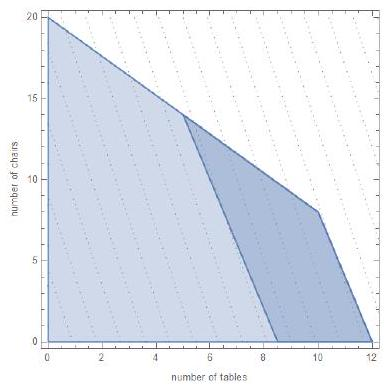
\includegraphics[width=0.5\textwidth]{optimization/multi-objective/images/2022_02_28_634e8079070800ac7e3cg-10}
    \caption{Feasible set with revenue constrained to at least 70\% of the maximum.}
\end{figure}

This \emph{epsilon-constraint} method provides flexibility to explore trade-offs, generating new points on the Pareto frontier.

\paragraph{Pareto Optimality}

Many feasible solutions exist, but only some are \emph{Pareto optimal}. A solution is Pareto optimal if no other feasible solution improves one objective without worsening another.

\begin{definition}{Pareto Optimal}{}
Given a feasible set \(P\) and objective functions \(f_i: P \to \mathbb{R}\) to \emph{maximize}, a point \(\mathbf{x} \in P\) is \emph{Pareto Optimal} if there is no \(\overline{\mathbf{x}} \in P\) such that:
\[
\begin{aligned}
& f_i(\overline{\mathbf{x}}) > f_i(\mathbf{x}) \text{ for some } i, \\
& f_j(\overline{\mathbf{x}}) \ge f_j(\mathbf{x}) \text{ for all } j \ne i.
\end{aligned}
\]
That is, no objective can be strictly improved without sacrificing performance in at least one other. The \emph{Pareto Frontier} is the set of all such efficient points.
\end{definition}




\begin{figure}[h]
    \centering
    
            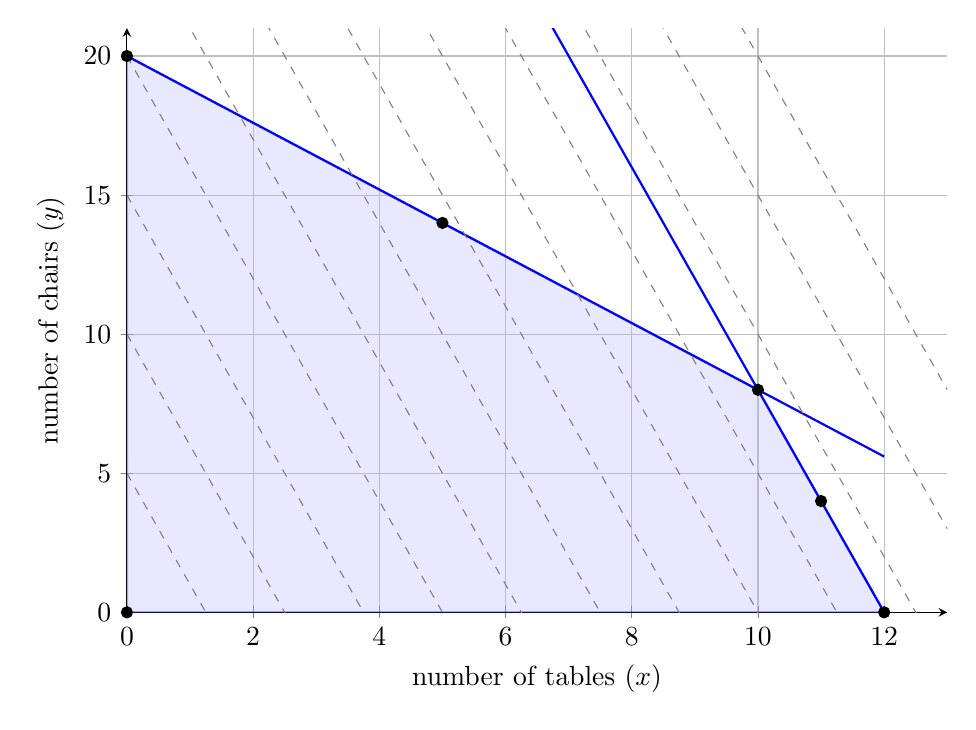
\begin{tikzpicture}
  \begin{axis}[
    xlabel={number of tables ($x$)},
    ylabel={number of chairs ($y$)},
    axis lines=left,
    xmin=0, xmax=13,
    ymin=0, ymax=21,
    xtick={0,2,4,6,8,10,12},
    ytick={0,5,10,15,20},
    width=12cm,
    height=9cm,
    grid=both,
    enlargelimits=false,
  ]

  % Feasible region (blue fill)
  \addplot[fill=blue!30, draw=blue, opacity = 0.3, thick] coordinates {
    (0,0)
    (0,20)
    (10,8)
    (12,0)
    (0,0)
  };
  
  % Constraint lines
  \addplot[domain=0:12, thick, blue] {48 - 4*x}; % 80x + 20y = 960
  \addplot[domain=0:12, thick, blue] {20 - 1.2*x}; % 12x + 10y = 200

  % Integer points in feasible region
  \foreach \pt in {
    (0,0), (0,20), (10,8), (12,0),
    (5,14), (11,4)
  } {
    \addplot[only marks, mark=*, mark size=2pt, black] coordinates {\pt};
  }
    % Objective function lines (example)
\foreach \z in {5,10,...,60}{
    \addplot[dashed,gray, domain=0:13, samples=2] {(\z - 4*x)};
}


  \end{axis}
\end{tikzpicture}

    %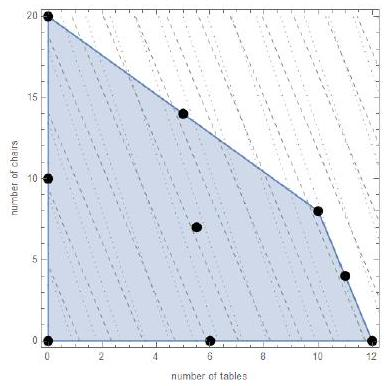
\includegraphics[width=0.5\textwidth]{optimization/multi-objective/images/2022_02_28_634e8079070800ac7e3cg-13}
    \caption{Identifying the Pareto frontier among possible solutions.}
\end{figure}


\paragraph{Summary of Multi-Objective Optimization Methods}

\begin{table}[h]
\centering
\caption{Summary of Multi-Objective Optimization Methods}
\renewcommand{\arraystretch}{1.3}
\begin{tabular}{|l|p{4.2cm}|p{3.5cm}|p{3.5cm}|}
\hline
\textbf{Method} & \textbf{Key Idea} & \textbf{Pros} & \textbf{Cons} \\
\hline
\textbf{Weighted Sum} & Combine objectives into a single scalar using a weighted sum & Simple and computationally efficient & May miss Pareto-optimal solutions in non-convex regions \\
\hline
\textbf{Lexicographic} & Prioritize objectives in strict order & Matches real-world decision hierarchies & Does not explore trade-offs or the full frontier \\
\hline
\textbf{Epsilon-Constraint} & Optimize one objective, treat others as constraints & Finds non-convex parts of the frontier & Requires repeated solves, hard to set $\varepsilon$ \\
\hline
\textbf{Goal Programming} & Minimize deviation from target values & Useful when goals are known & Sensitive to target and weight choices \\
\hline
\end{tabular}
\end{table}



\paragraph{Goal Programming}
Goal Programming allows you to set specific targets (goals) for each objective and minimize the weighted sum of deviations from these goals. It generalizes the idea of rollover benchmarks by specifying multiple constraints in a flexible way.

\paragraph{Epsilon-Constraint Method}
One can maximize one objective while turning the other objectives into constraints (with adjustable right-hand sides). Varying those constraints systematically reveals the entire Pareto front.

\begin{figure}[h]
    \centering
    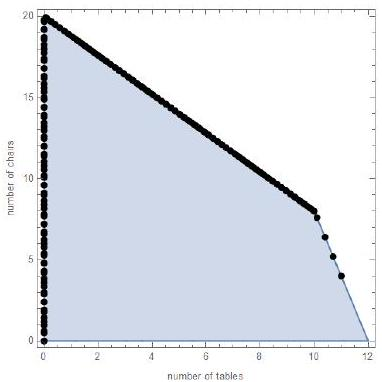
\includegraphics[width=0.5\textwidth]{optimization/multi-objective/images/2022_02_28_634e8079070800ac7e3cg-14}
    \caption{Pareto frontier with respect to original design variables.}
\end{figure}

In practice, it is often more natural to plot the frontier with respect to the \emph{objectives} rather than the decision variables:

\begin{figure}[h]
    \centering
    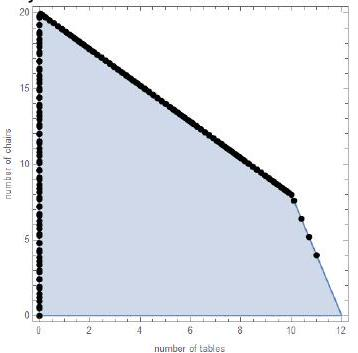
\includegraphics[width=0.5\textwidth]{optimization/multi-objective/images/2022_02_28_634e8079070800ac7e3cg-15}
    \caption{Pareto frontier plotted in (Objective\_1, Objective\_2)-space.}
\end{figure}

\subsection{Where Are Pareto Frontiers Useful?}

The furniture example provided earlier illustrated the basic idea of trading off two objectives. 
In practice, \emph{Pareto frontiers} are a core tool in decision-making across disciplines, enabling analysts to understand the trade-off structure of a problem before committing to a single solution. 
They are particularly valuable in settings where:
\begin{itemize}
    \item Stakeholders value different objectives in different ways, and no single objective can be optimized without affecting others.
    \item There is uncertainty or disagreement about the correct weighting of objectives, making it desirable to present a range of compromise solutions.
    \item The decision-making process is iterative and interactive, allowing exploration of “what if” scenarios.
\end{itemize}

Some common application areas include:

\begin{itemize}
    \item \textbf{Political Redistricting} -- balancing compactness, fairness in representation, community preservation, and compliance with legal constraints.
    \item \textbf{Portfolio Optimization} -- selecting asset allocations that balance expected return and risk, often with additional objectives such as liquidity or ethical constraints.
    \item \textbf{Engineering Design} -- optimizing multiple performance metrics simultaneously (e.g., fuel efficiency vs.\ speed vs.\ structural weight).
    \item \textbf{Sustainable Construction} -- minimizing environmental impact while meeting cost and performance requirements.
    \item \textbf{Public Policy Planning} -- balancing efficiency, equity, and resilience in transportation, healthcare, or energy systems.
\end{itemize}

\subsubsection{Political Redistricting}
In political redistricting, objectives such as \emph{district compactness} and \emph{minority representation} can conflict. A highly compact district might not adequately represent certain communities, while ensuring strong representation may require irregular shapes. A Pareto frontier can reveal feasible trade-offs before a final plan is chosen.
\begin{figure}[h]
    \centering
    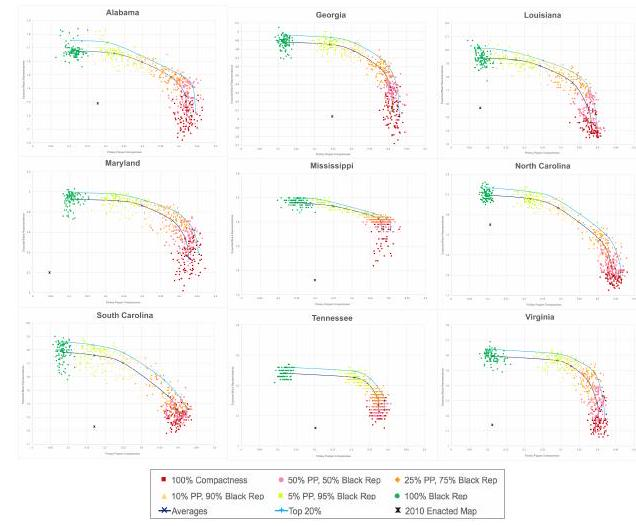
\includegraphics[width=0.5\textwidth]{optimization/multi-objective/images/2022_02_28_634e8079070800ac7e3cg-19}
    \caption{Balancing compactness and representation in districting.}
\end{figure}

\subsubsection{Portfolio Optimization}
In finance, the Pareto frontier corresponds to the \emph{efficient frontier} -- portfolios that achieve the lowest possible risk for a given expected return, or the highest return for a given risk. The curve helps investors choose a portfolio consistent with their risk tolerance.
\begin{figure}[h]
    \centering
    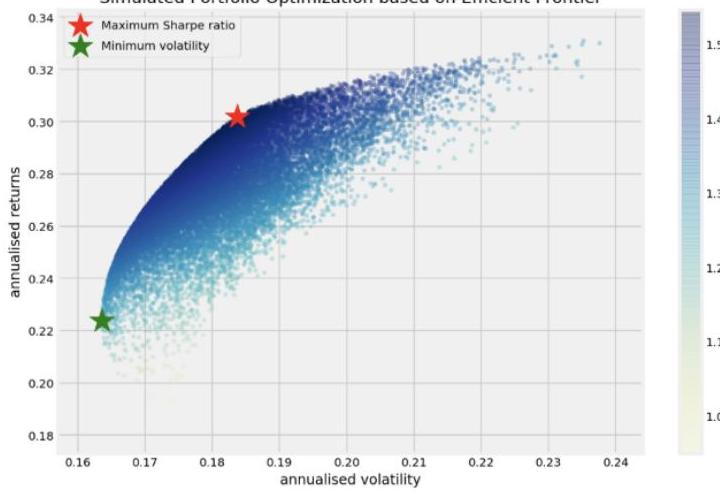
\includegraphics[width=0.5\textwidth]{optimization/multi-objective/images/2022_02_28_634e8079070800ac7e3cg-20}
    \caption{Risk-return trade-off curve (efficient frontier).}
\end{figure}

\subsubsection{Aircraft Design}
Aircraft design involves competing goals: reducing weight improves fuel efficiency but may reduce structural strength; improving speed may increase cost and reduce range. Multi-objective optimization helps identify designs that balance these trade-offs.
\begin{figure}[h]
    \centering
    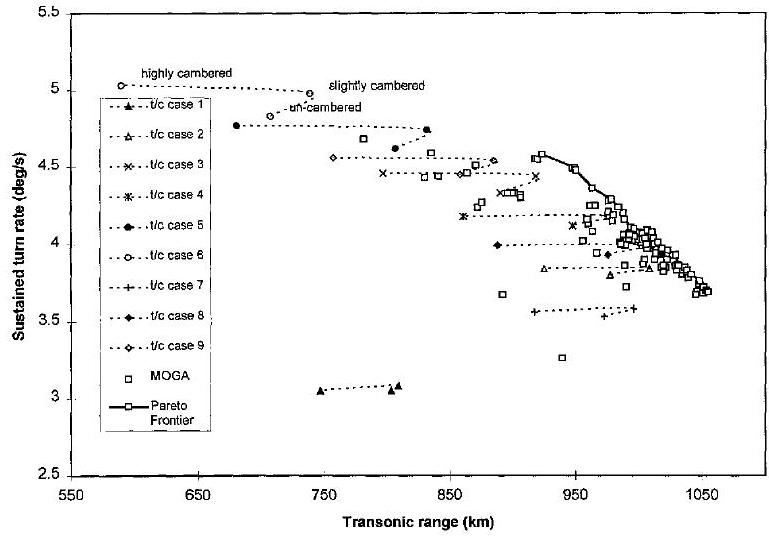
\includegraphics[width=0.5\textwidth]{optimization/multi-objective/images/2022_02_28_634e8079070800ac7e3cg-21}
    \caption{Pareto frontier of design objectives for aircraft wings.}
\end{figure}

\subsubsection{Vehicle Dynamics}
In vehicle performance tuning, engineers might balance acceleration, cornering stability, and fuel efficiency. Pareto frontiers reveal how improving one aspect affects the others, supporting design decisions or consumer product differentiation.
\begin{figure}[h]
    \centering
    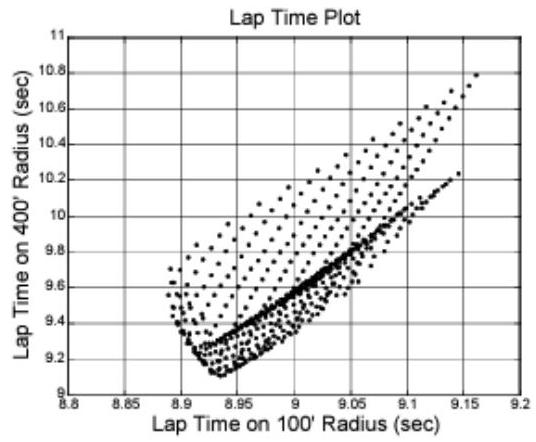
\includegraphics[width=0.5\textwidth]{optimization/multi-objective/images/2022_02_28_634e8079070800ac7e3cg-22}
    \caption{Trade-off surface for vehicle performance metrics.}
\end{figure}

\subsubsection{Sustainable Construction}
In sustainable building design, cost, energy efficiency, carbon footprint, and occupant comfort are all relevant. Pareto frontiers provide transparency in how design changes affect these factors, helping teams reach consensus.
\begin{figure}[h]
    \centering
    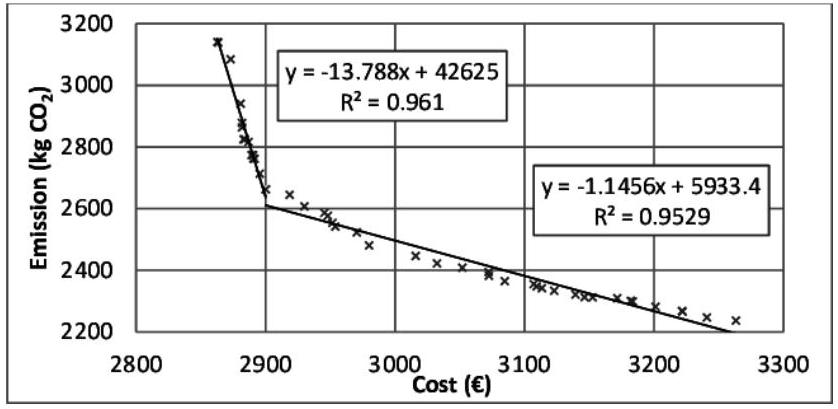
\includegraphics[width=0.5\textwidth]{optimization/multi-objective/images/2022_02_28_634e8079070800ac7e3cg-23}
    \caption{Multi-objective trade-offs in a sustainable design context.}
\end{figure}

\paragraph{Other Notable Application Domains}
\begin{itemize}
    \item \emph{Healthcare}: Balancing treatment effectiveness, side effects, and cost in medical decision-making.
    \item \emph{Energy Planning}: Managing trade-offs between cost, reliability, and environmental impact in power generation.
    \item \emph{Machine Learning}: Simultaneously optimizing prediction accuracy and model interpretability or energy consumption.
    \item \emph{Supply Chain Design}: Balancing delivery time, inventory cost, and resilience to disruptions.
\end{itemize}

These examples illustrate the broad applicability of Pareto analysis: it is not just a theoretical tool, but a practical decision-support method in domains where competing objectives are the norm rather than the exception.


\subsection{Where Are Pareto Frontiers Useful?}

Although our furniture example was straightforward, multi-objective optimization methods are fundamental in many areas:

\begin{itemize}
    \item \textbf{Political Redistricting} (e.g., balancing fairness vs.\ compactness)
    \item \textbf{Portfolio Optimization} (balancing risk vs.\ return)
    \item \textbf{Aircraft/Vehicle Design} (trade-offs between fuel efficiency, cost, speed, etc.)
    \item \textbf{Sustainability in Construction} (minimizing environmental impact vs.\ cost)
\end{itemize}

\subsubsection{Political Redistricting}
\begin{figure}[h]
    \centering
    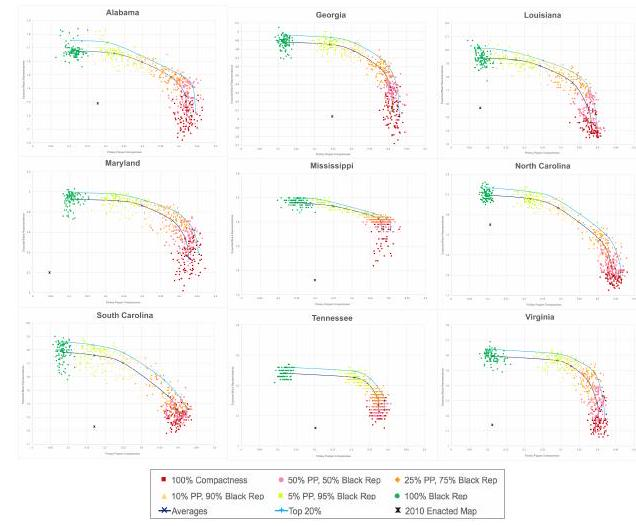
\includegraphics[width=0.5\textwidth]{optimization/multi-objective/images/2022_02_28_634e8079070800ac7e3cg-19}
    \caption{Balancing multiple objectives (compactness, representation, etc.) in districting.}
\end{figure}

\subsubsection{Portfolio Optimization}
\begin{figure}[h]
    \centering
    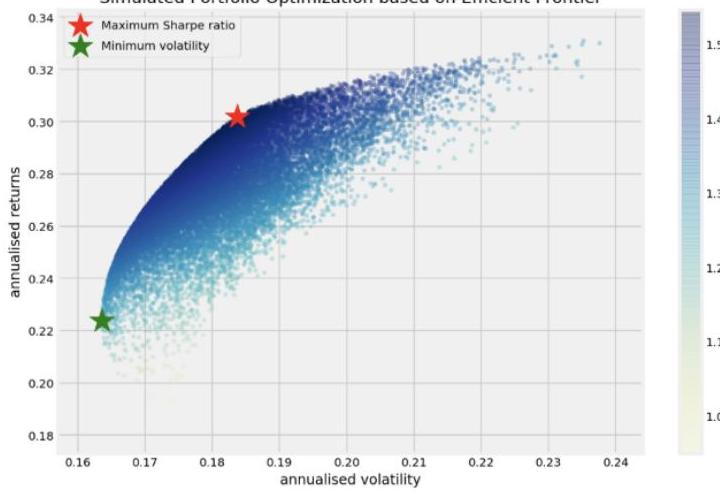
\includegraphics[width=0.5\textwidth]{optimization/multi-objective/images/2022_02_28_634e8079070800ac7e3cg-20}
    \caption{Risk-Return trade-off curve known as the Efficient Frontier.}
\end{figure}

\subsubsection{Aircraft Design }
\begin{figure}[h]
    \centering
    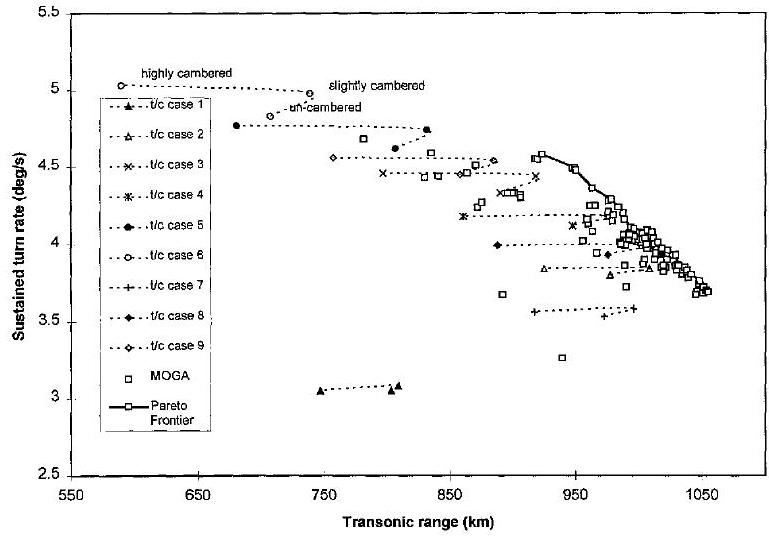
\includegraphics[width=0.5\textwidth]{optimization/multi-objective/images/2022_02_28_634e8079070800ac7e3cg-21}
    \caption{Pareto frontier of various design objectives for aircraft wings.}
\end{figure}

\subsubsection{Vehicle Dynamics }
\begin{figure}[h]
    \centering
    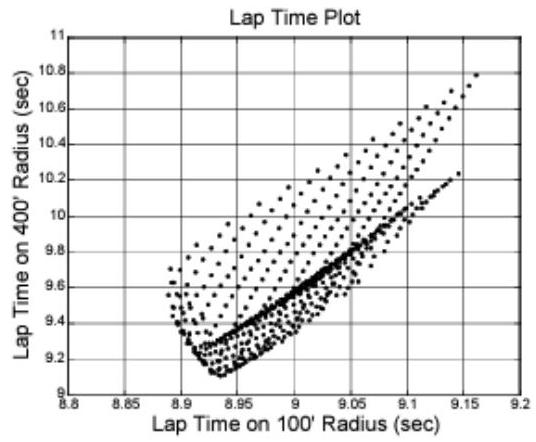
\includegraphics[width=0.5\textwidth]{optimization/multi-objective/images/2022_02_28_634e8079070800ac7e3cg-22}
    \caption{Grid search results in the vehicle performance space.}
\end{figure}

\subsubsection{Sustainable Construction}
\begin{figure}[h]
    \centering
    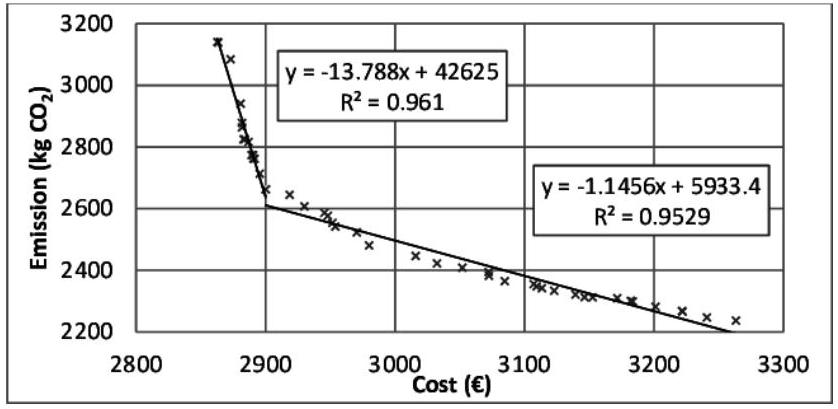
\includegraphics[width=0.5\textwidth]{optimization/multi-objective/images/2022_02_28_634e8079070800ac7e3cg-23}
    \caption{Multi-objective trade-offs in a sustainable design context.}
\end{figure}

\section{Brief Introduction to \texttt{pymoo}}
\label{sec:pymoo}

\begin{resource}
\href{https://pymoo.org/}{Python Multi Objective Optimization (Pymoo)}
\end{resource}

\texttt{pymoo} is a Python-based framework for multi-objective optimization. It supports multiple algorithms (e.g., NSGA-II, MOEA/D, etc.), visualization of Pareto fronts, and easy experimentation with custom problems.

\medskip
\noindent
\textbf{Example (Scalarization Approach in \texttt{pymoo}):}
\begin{verbatim}
pip install pymoo
\end{verbatim}

\begin{verbatim}
from pymoo.factory import get_problem, get_algorithm, get_reference_directions
from pymoo.optimize import minimize

# Example: Using a built-in multi-objective problem
problem = get_problem("zdt1")

# Use a standard evolutionary algorithm
algorithm = get_algorithm("nsga2", pop_size=100)

# Run the optimization
res = minimize(problem, algorithm, ("n_gen", 200), seed=1, verbose=False)

# res.X are decision variables, res.F are the objectives
print("Pareto Approximation:", res.F)
\end{verbatim}

This snippet illustrates how straightforward it can be to generate an approximate Pareto front using existing libraries.

\section{References}

\begin{itemize}
    \item[\textbf{[1]}] S. Fenwick and John C. Harris. \emph{The Application of Pareto Frontier Methods in the Multidisciplinary Wing Design of a Generic Modern Military Delta Aircraft}: Semantic Scholar, Jan 1999.  
    \\
    \url{https://WWW.semanticscholar.org/paper/The-application-of-Pareto-frontier-methods-in-the-a-Fenwick-Harris/fced00a59d200c2c74ed655a457344bcleea6ff5.}

    \item[\textbf{[2]}] T. Garc\'ia-Segura, V. Yepes, and J. Alcal\'a. \emph{Sustainable Design Using Multiobjective Optimization of High-Strength Concrete I-Beams}. In \emph{The 2014 International Conference on High Performance and Optimum Design of Structures and Materials HPSM/OPTI}, volume 137, pages 347--358, 2014.  
    \\
    \url{https://www.researchgate.net/publication/271439836_Sustainable_design_using_multiobjective_optimization_of_high-strength_concrete_l-beams.}

    \item[\textbf{[3]}] Nicholas Goedert, Robert Hildebrand, Laurel Travis, Matthew Pierson, and Jamie Fravel. \emph{Black Representation and District Compactness in Southern Congressional Districts.} Not yet published; ask Dr. Hildebrand for it.

    \item[\textbf{[4]}] Edward M. Kasprzak and Kemper E. Lewis. \emph{Pareto Analysis in Multiobjective Optimization Using the Collinearity Theorem and Scaling Method.} Structural and Multidisciplinary Optimization.

    \item[\textbf{[5]}] Ricky Kim. \emph{Efficient Frontier Portfolio Optimisation in Python}, June 2021.  
    \\
    \url{https://towardsdatascience.com/efficient-frontier-portfolio-optimisation-in-python-e7844051e7f.}
\end{itemize}
